\section{Verfahrensweisen und wesentliche Gestaltungsprinzipien}\label{sec:methodenGrundlage}
Um eine einheitliche Auffassung der Charakteristika dynamischer Geschäftsprozesse zu beschrieben, wird der inhaltliche Rahmen der Bachelorarbeit zunächst dargelegt.
Da sich die Entwicklung der Methode an fundamentalen Ansätzen der Softwareentwicklung orientiert, werden nachfolgend dessen Grundlagen dargestellt, um die wesentlichen Gestaltungselemente der Methode in Erfahrung zu bringen. Danach werden die Konzepte von Lean Management charakterisiert, auf die sich die Methode insbesondere bei der Modellierung auf der Geschäftsprozessebene stützt.

\subsection{Charakterisierung dynamischer Geschäftsprozesse}
Die Auffassung dynamischer Geschäftsprozesse im Rahmen dieser Bachelorarbeit versteht diese so, dass sich deren Ablauf, als unmittelbare und automatisierte Reaktion auf Ereignisse, in Echtzeit anpassen kann. Gemäß Abbildung \ref{fig:Grundlegender architektonischer Entwurf einer EDA} werden die zugehörigen Ereignisverarbeitungsregeln zur Echtzeitverarbeitung der relevanten Ereignisse und deren Beziehungen untereinander ausschließlich auf der Ereignisverarbeitungsebene implementiert, während die Kommunikation mit der Geschäftsprozessebene einzig mittels Ereignissen durch einen Ereignisverarbeitungsdienst abläuft.
\cite{Vidackovic.2014}

Die unmittelbare Reaktion auf ein solches Ereignis auf Geschäftsprozessebene soll sich im Rahmen der Modellierungsmöglichkeiten von \ac{BPMN} 2.0 bewegen, sodass der Fokus hier auf der Modellierung automatisierbarer Geschäftsprozesse in der Entwurfsphase liegt mit der wesentlichen Eigenschaft, auf eintretende Ereignisse möglichst dynamisch reagieren zu können. Die Dynamik solcher ereignisgesteuerter Geschäftsprozesse basiert demnach auf der Ereignisverarbeitung auf der Ereignisverarbeitungsebene, während der Ablauf der Geschäftsprozesse mit ausreichender Flexibilität auf der Geschäftsprozessebene ausgestattet sein muss, um die von der Ereignisverarbeitung angestoßenen Aktivitäten als Reaktion in Echtzeit aufgetretenen Ereignisse realisieren zu können.

\subsection{Grundlagen der Softwareentwicklung}
Ein wesentliches Ziel dieser Bachelorarbeit ist die Umsetzung des konzipierten Geschäftsprozesses in Form von Software. Daher wird an dieser Stelle zunächst der Begriff Software selbst spezifiziert.

Laut \citeauthor{Balzert.2009} umfasst der Begriff \textit{Software} sowohl die Programme und Daten, als auch entsprechende Dokumentationen, die zur Anwendung der Software benötigt werden. Des Weiteren beschreibt er ein \textit{Softwaresystem}, das ein wesentlicher Bestandteil eines jeden modernen Informationssystems ist, als eine Ansammlung von Komponenten und Elementen, die wiederum aus Software bestehen. Softwaresysteme werden noch weiter unterteilt in Anwendungssoftware und Systemsoftware, wobei Systemsoftware grundsätzlich das Betriebssystem, in der Praxis aber auch den Compiler, Datenbanken, Kommunikationsprogramme und Dienstprogramme umfasst.
\cite{Balzert.2009}
Anwendungssoftware ist Software, die Tätigkeiten eines Anwenders durch die Unterstützung von \ac{IT} unterstützen sollen. 
Anwendungssoftware nutzt in der Regel wesentliche Funktionalitäten der zugrunde liegenden Systemsoftware. Der Fokus der Softwareentwicklung in der vorliegenden Bachelorareit liegt auf der Entwicklung von Anwendungssoftware. 
\cite{Balzert.2009}
Die Softwareentwicklung als Ganzes betrachtet orientiert sich an der Zielsetzung, Softwaresysteme durch den systematischen Einsatz von Prinzipien, Vorgehensweisen und Werkzeugen für die Herstellung und Anwendung von Software.
\cite{Balzert.2009}
Bei der Softwareentwicklung, englisch \textit{Software-Engineering}, handelt es sich folglich, um eine ingenieurmäßige Vorgehensweise, da es sie eine die Schaffung von möglichst erffektiven sowie effizienten Lösungen für konkrete und praktische Problemstellungen.
\cite{Balzert.2009}

Im Laufe der Zeit sind die Softwaresysteme weit vorangeschritten, wodurch auch die Komplexität im den Softwareentwicklungsprojekten stetig wächst. Heute sind iterative und agile Eigenschaften in einem Vorgehensmodell für komplexe Softwaresysteme kaum wegzudenken. Beispiele hierzu sind das \textit{Wasserfallmodell, V-Modell, Extreme Programming oder Scrum}, da diese Vorgehensmodelle jedoch zu komplex für eine softwaretechnische Implementierung im Rahmen dieser Bachelorarbeit sind, wird an dieser Stelle von einer expliziten Betrachtung der einzelnen Modelle abgesehen und es wird der Ansatz verfolgt die notwendigen Gemeinsamkeiten darzustellen.
\cite{Krypczyk.2018}

Im Wesentlichen umfasst ein jedes Vorgehensmodell zur Entwicklung von Software die drei, in Abbildung \ref{fig:Phasen der Softwareentwicklung} dargestellten, Phasen: \textit{Analyse, Entwurf und Implementierung}

\begin{figure}[H]
	\centering 
    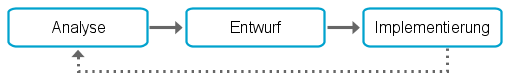
\includegraphics[width=\textwidth]{img/entwicklung.png}	
    \caption[Phasen der Softwareentwicklung]
    {Phasen der Softwareentwicklung\protect\footnotemark}
    \label{fig:Phasen der Softwareentwicklung}
\end{figure}
\footnotetext{Eigene Darstellung}
\footnotetext{Die Abbildung dient lediglich der Visualisierung und ist nicht \ac{BPMN} 2.0 konform.}

Die Analysephase beschäftigt sich eingehend damit welche erfolgskritischen Anforderungen an die zu erstellende Software existieren. Dabei erfolgt eine explizite Betrachtung der Ausgangslage, um die Probleme, die es mit Hilfe der Software zu lösen oder zu unterstützen gilt, zu identifizieren. Sind die wesentlichen Anforderungen zusammengetragen, werden Maßnahmen zur Problembehandlung erörtert und ausgewählt. Anschließend erfolgt der grundlegende Architekturentwurf der Software. In der letzten Phase, der Implementierung, wird die entworfene Software letzendlich in eine ausführbare Version transformiert. Die Aufgaben der Implementierung umfassen die Erstellung von Benutzerschnittstellen, die Erarbeitung der notwendigen Geschäftslogik und die Umsetzung der Datenhaltung in Form von Datenbanken oder Schnitttstellen zu weiterführender Software. Diese Phasen können bei Bedarf beliebig oft wiederholt werden.
\cite{Krypczyk.2018}

Als bewährte Methode für diesen Minimalansatz der Softwareentwicklung wird im Rahmen dieser Bachelorarbeit das \textit{Design-Thinking} herangezogen. 
\cite{Elsner.2018}
Design-Thinking ist eine Methode, um zielorientiert Lösungen zu finden, die aus Anwendersicht gewünscht sind. Die Phasen des Design-Thinking-Prozesses heißen \textit{Discover, Design und Deliver}, die als Synonym zu den Phasen \textit{Analyse, Entwurf und Implementierung} angesehen werden dürfen. Ziel dieser Form der Softwareentwicklung ist es möglichst zeitnahe an einen funktionsfähiges Produkts zu gelangen.

Im Zusammenhang mit dieserart Vorgehensmodellen hört man daher oft den Begriff \ac{MVP}. Ein \ac{MVP}, wörtlich ein minimales, überlebensfähiges Produkt, ist die erste Version eines Produkts, die entwickelt werden muss, um mit minimalem Aufwand die Mindestanforderungen eines Bedarfs zu decken. Das \ac{MVP} muss bereits insofern funktionsfähig sein, dass es vom Anwendern getestet werden kann.
\cite{Elsner.2018}
Die in dieser Bachelorarbeit konzipierte Methode orientiert sich an den grundlegenden Phasen der Softwareentwicklung, sowie den Prinzipien von Design-Thinking. 

\subsection{Lean Management}

Lean Management beschäftigt sich mit der Effizienz und Effektivität von Geschäftsprozessen. Jede Art von Verschwendung steht der Effizienz und Effektivität entgegen und muss daher vermieden werden.
Der Begriff \textit{Lean Management} beschreibt ein System, das vielfältige Ansätze und Philosophien miteinander verbindet, um Geschäftsprozessen im gesamten Unternehmen dadurch wertschöpfender zu gestalten, dass die Verschwendung von Ressourcen erkannt und eliminiert wird.
Lean Management beinhaltet sowohl organisatorische Prinzipien, operative Strategien zur Erfüllung des Unternehmensziele, betriebswirtschaftliche Maßnahmen, aber auch Vorgaben an die einzelnen Angestellten.
\cite{Schell.2017}

Der Ursprung der heutigen Philosophie des \textit{Lean Management} liegt in Japan. Im wirtschaftlich angeschlagenen Japan der Nachkriegszeit des Zweiten Weltkriegs herrschte vor allem in den Industrieunternehmen ein akuter Ressourcenmangel, da Japan in diesen Jahren keine Wirtschaftshilfe von anderen Ländern erhielt. In dieser Notsituation mussten die Industrieunternehmen ihre Ressourcen schonend einsetzen, Verschwendung vermeiden, Prozesse optimieren und gleichzeitig die für den Markt notwendige Qualität liefern.
Mit dieser Herausforderung konfrontiert, entstand bei der Firma Toyota das \textit{Toyota-Produktionssystem}, der Vorreiter von Lean Management.
\cite{Morgan.2006}

Grundsätzlich werden unter Verschwendung alle Aktivitäten und Ressourcen verstanden, die nicht zur Wertschöpfung eines Industriesbetriebs beitragen. Diese nicht wertschöpfenden Tätigkeiten werden als überflüssig angesehen und sind zu eliminieren.
Das \textit{Toyota-Produktionssystem} kennt 7 Arten der Verschwendung. Die unterschiedlichen Arten von Verschwendung werden in Tabelle \ref{tab:Arten von Verschwendung} dargestellt.

\begin{table}[H]
	\centering
	\begin{tabularx}{\textwidth}{l X} 
		\toprule
		\textbf{Art}  &   
		\textbf{Beschreibung}  \\ 		\midrule
		
		Bewegung &   
		Lange Laufwege und umständliche Aktivitäten  \\  \cmidrule(r){1-1} \cmidrule(r){2-2}
		
		Defekte &   
		Qualitätsmängel der Produkte \\ \cmidrule(r){1-1} \cmidrule(r){2-2}
		
		Lagerbestand &   
		Umlaufbestände oder Lager mit fertigen Produkten  \\ \cmidrule(r){1-1} \cmidrule(r){2-2}
		
		Transport &   
		Häufige Transporte von Ressourcen  \\ \cmidrule(r){1-1} \cmidrule(r){2-2}
		
		Überproduktion &   
	    Herstellung nicht benötigter Produkte \\ \cmidrule(r){1-1} \cmidrule(r){2-2}
		
		Unnötige Prozesse &   
		Prozesse oder Fertigungsverfahren ohne Notwendigkeit  \\ \cmidrule(r){1-1} \cmidrule(r){2-2}
		
		Warten &   
		Verzögerung bei den Tätigkeiten  \\
	    \bottomrule
	\end{tabularx}
	\caption{\label{tab:Arten von Verschwendung}Arten von Verschwendung}
\end{table}

\newpage

Aus der Lean-Philosophie lassen sich fünf wesentliche Prinzipien ableiten, die das Fundament für den Gebrauch von Lean Management bilden: \textit{Kundennutzen, Wertstrom, Fluss-Prinzip, Pull-Prinzip und Null Fehler}\begin{itemize}
    \item 
    Der \textbf{Kundennutzen} im Mittelpunkt stellt in der Lean-Philosophie eine fundamentale Leitlinie dar. 
    Es ist somit notwendig, mit den Kunden im Dialog zustehen, um die Bedürfnisse dieser verstehen zu können.
    \cite{Muller.2011} 
    \item
    Die \textbf{Wertstromanalyse} dient zur Identifizierung relevanter Stellen im Geschäftsprozess, die einen Beitrag zur Wertschöpfung leisten. Der Wertstrom wird durch alle Aktivitäten und Ereignisse gekennzeichnet, die für das Produkt notwendig ist. 
    \item
    Im Rahmen des \textbf{Fluss-Prinzips} wird, versucht die einzelnen Aktivitäten in einer optimalen Abfolge anzuordnen. Eine optimale Abfolge von Aktivitäten eines Geschäftsprozesses wird dann als nicht gegeben betrachtet, wenn es zu Wartezeiten oder Engpässen kommt.
    \item
    Das \textbf{Pull-Prinzip} beschreibt denselben Grundsatz wie die Kundeneinzelfertigung in der Produktionsplanung und -steuerung in SAP S/4HANA Cloud. Eine Fertigung darf nur erfolgen, wenn ein konkreter Bedarf durch einen Kundenauftrag existiert.
    \item
    Lean Management definiert einen Fehler als Abweichung von einem definierten Standard. Daher müssen für Geschäftsprozesse solche Toleranzgrenzen als Regeln definiert werden, um mögliche Fehler und daraus abgeleitete Qualitätsmerkmale zu ermitteln. Dieser Gedanke wird als \textbf{Null-Fehler-Prinzip} bezeichnet.
    Die Verantwortung für die Fehlererfassung und -behebung liegt bei den verantwortlichen Mitarbeitern.
\end{itemize}

Die Leitgedanken von Lean Management dienen in der vorliegenden Bachelorarbeit als Gedankenstütze bei der Identifizierung geeigneter Maßnahmen gegen Verschwendung und für Automatisierung und Reaktionsfähigkeit in der Fertigungsdurchführung mit SAP S/4HANA Cloud.